\section{Distributions of input variables for the global BDT}

\begin{figure}
    \centering
    \begin{subfigure}[b]{0.48\textwidth}
        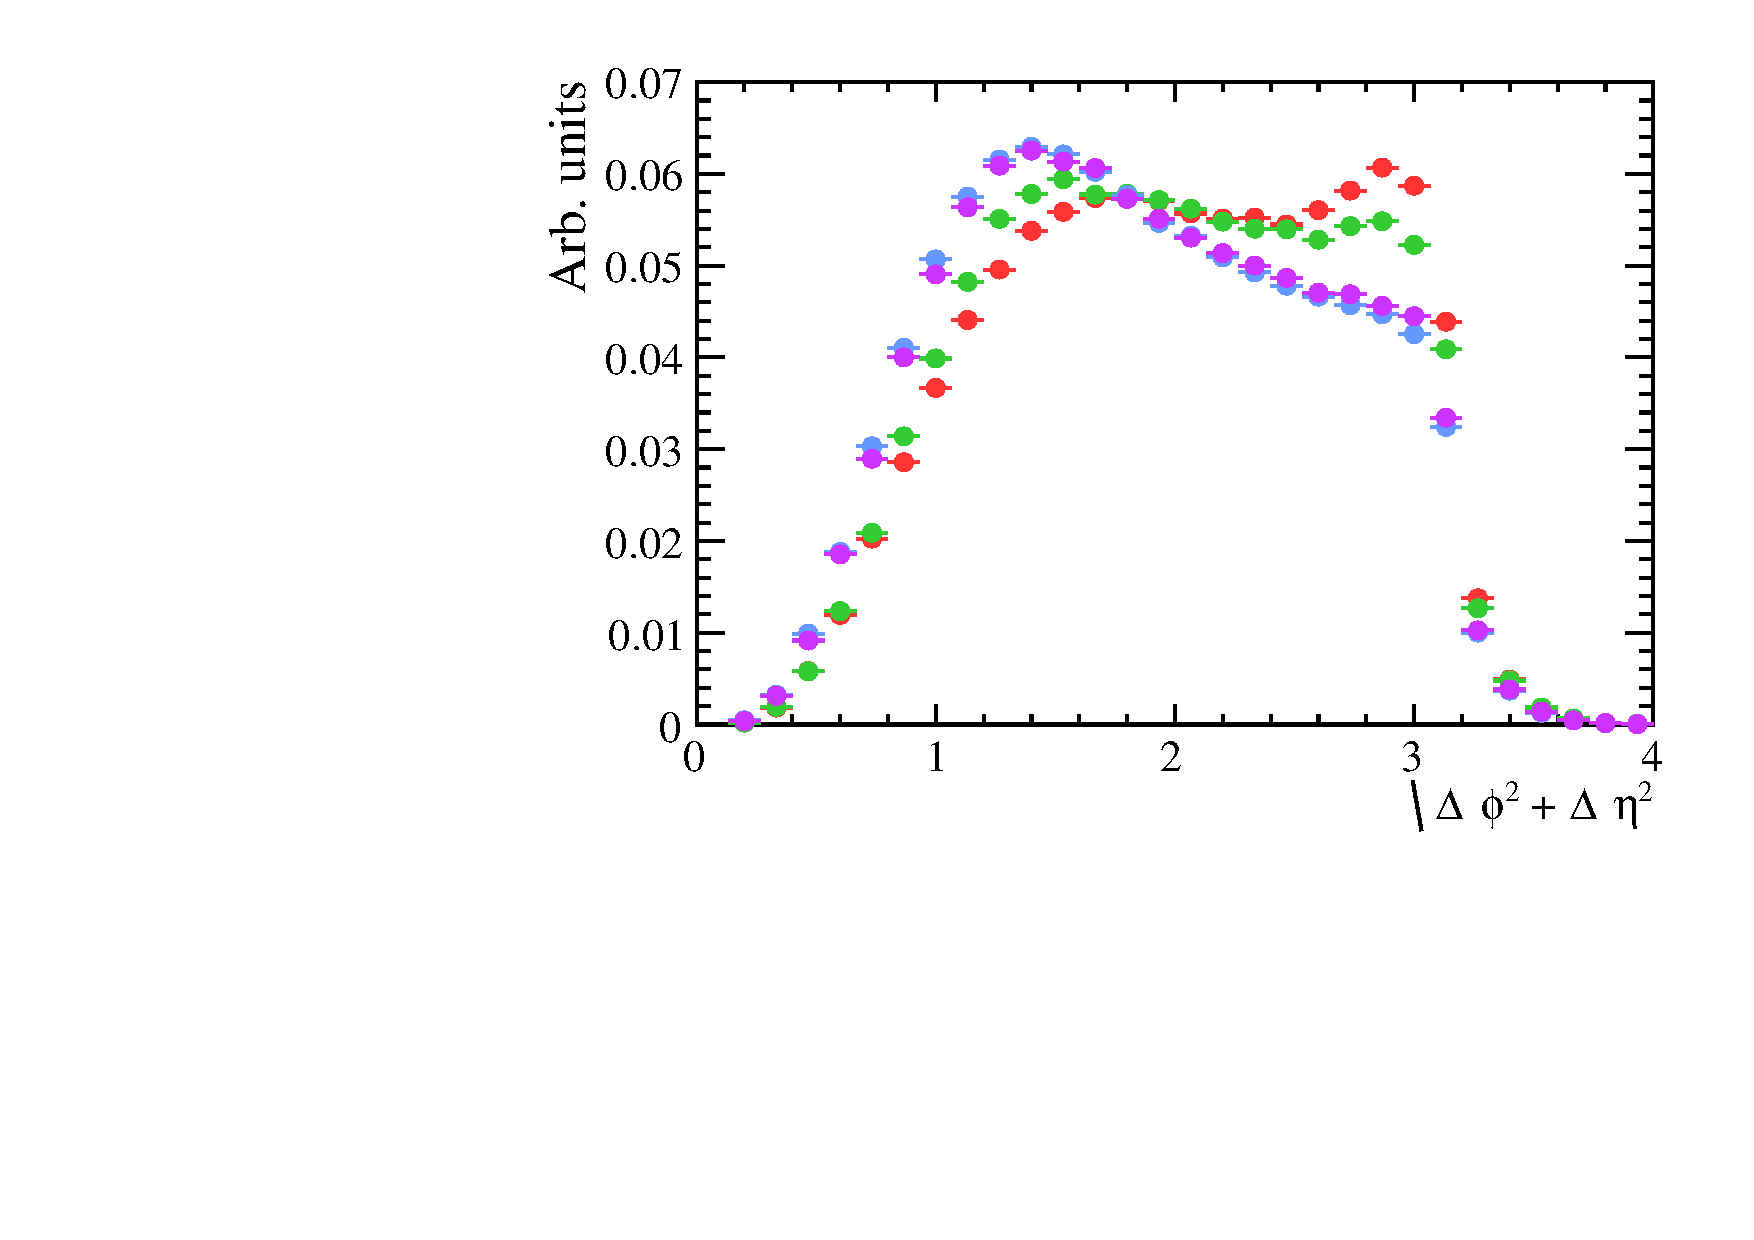
\includegraphics[width=\textwidth]{./Figs/Selection/signal_deltaR.pdf}
        \caption{ }
        \label{fig:BDTsig}
    \end{subfigure}
    ~ %add desired spacing between images, e. g. ~, \quad, \qquad, \hfill etc. 
      %(or a blank line to force the subfigure onto a new line)
    \begin{subfigure}[b]{0.48\textwidth}
       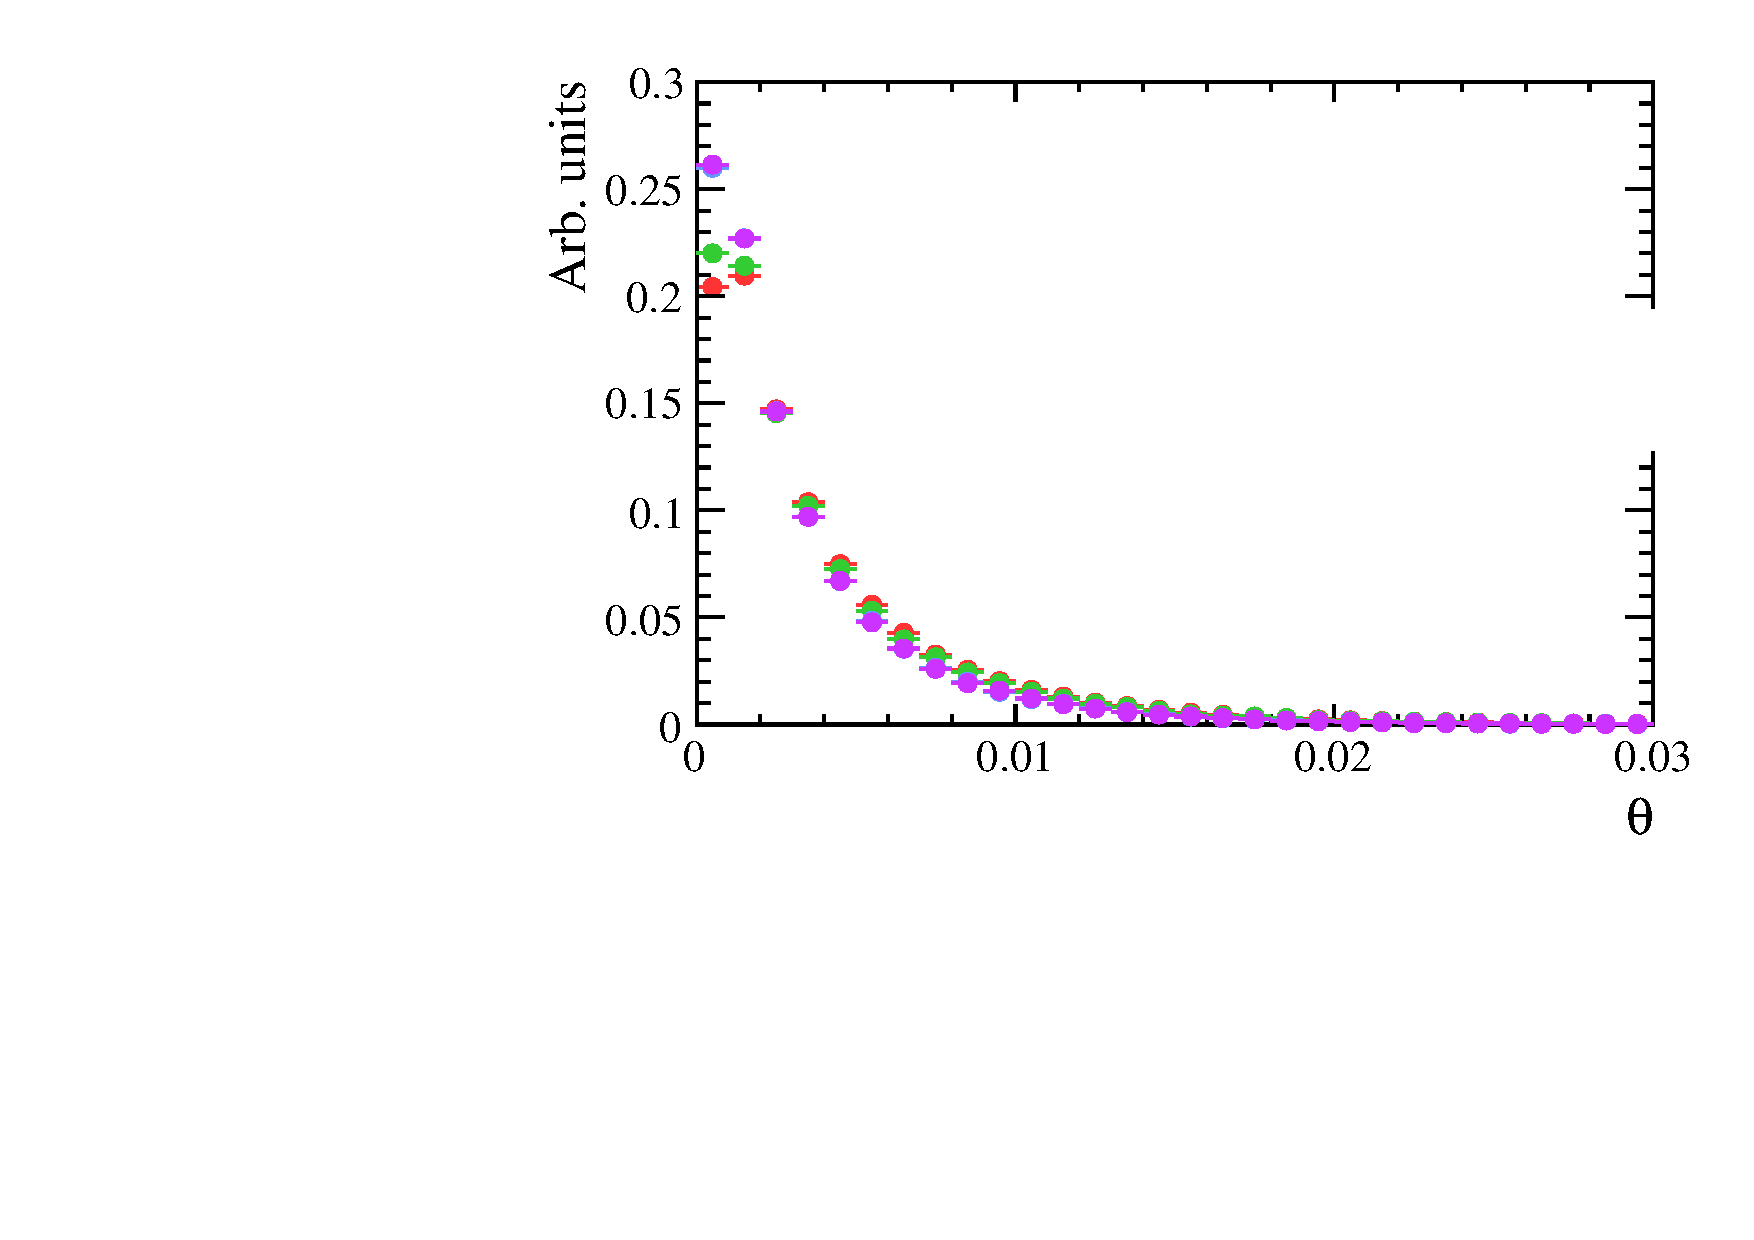
\includegraphics[width=\textwidth]{./Figs/Selection/signal_DIRA.pdf}
        \caption{ }
        \label{fig:BDTbkg}
    \end{subfigure}



 \begin{subfigure}[b]{0.48\textwidth}
        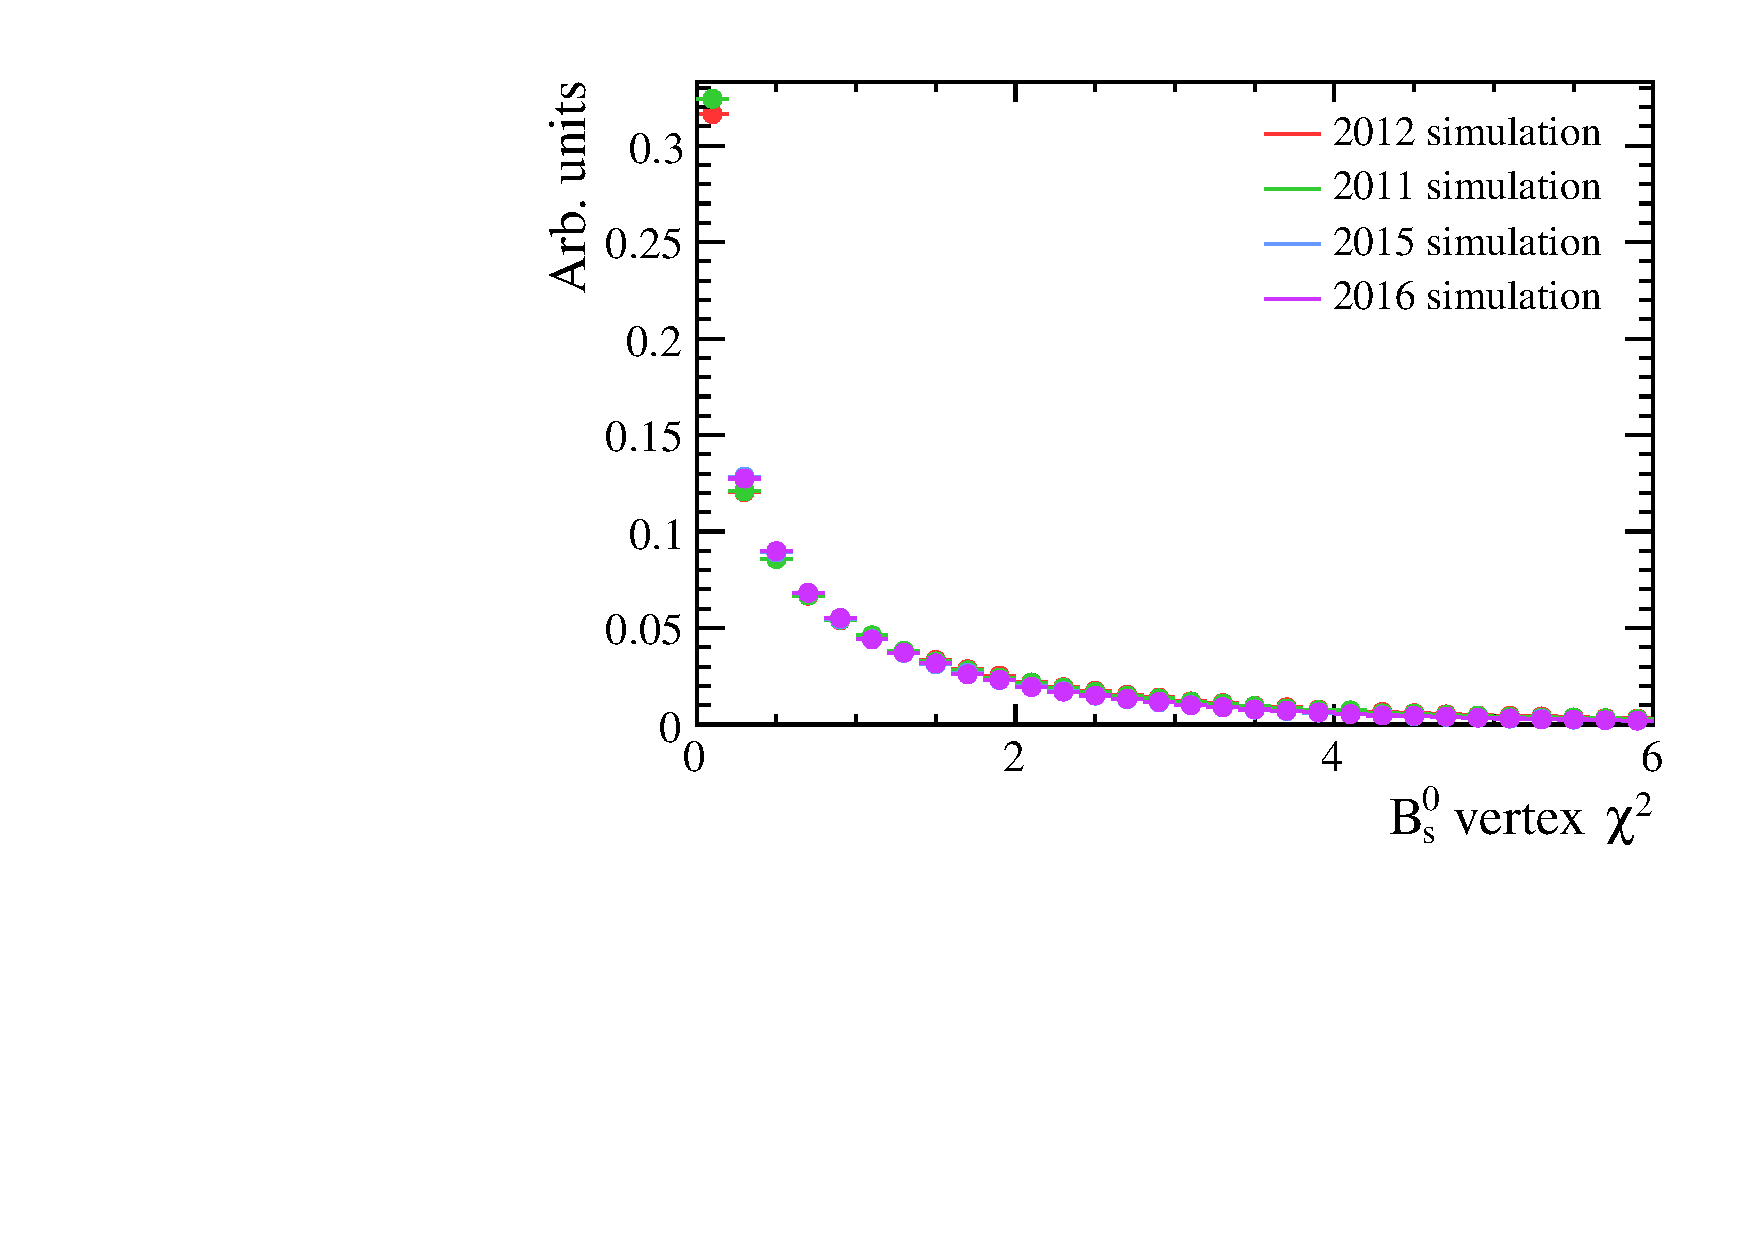
\includegraphics[width=\textwidth]{./Figs/Selection/signal_end_vertex.pdf}
        \caption{ }
        \label{fig:BDTsig}
    \end{subfigure}
    ~ %add desired spacing between images, e. g. ~, \quad, \qquad, \hfill etc. 
      %(or a blank line to force the subfigure onto a new line)
    \begin{subfigure}[b]{0.48\textwidth}
       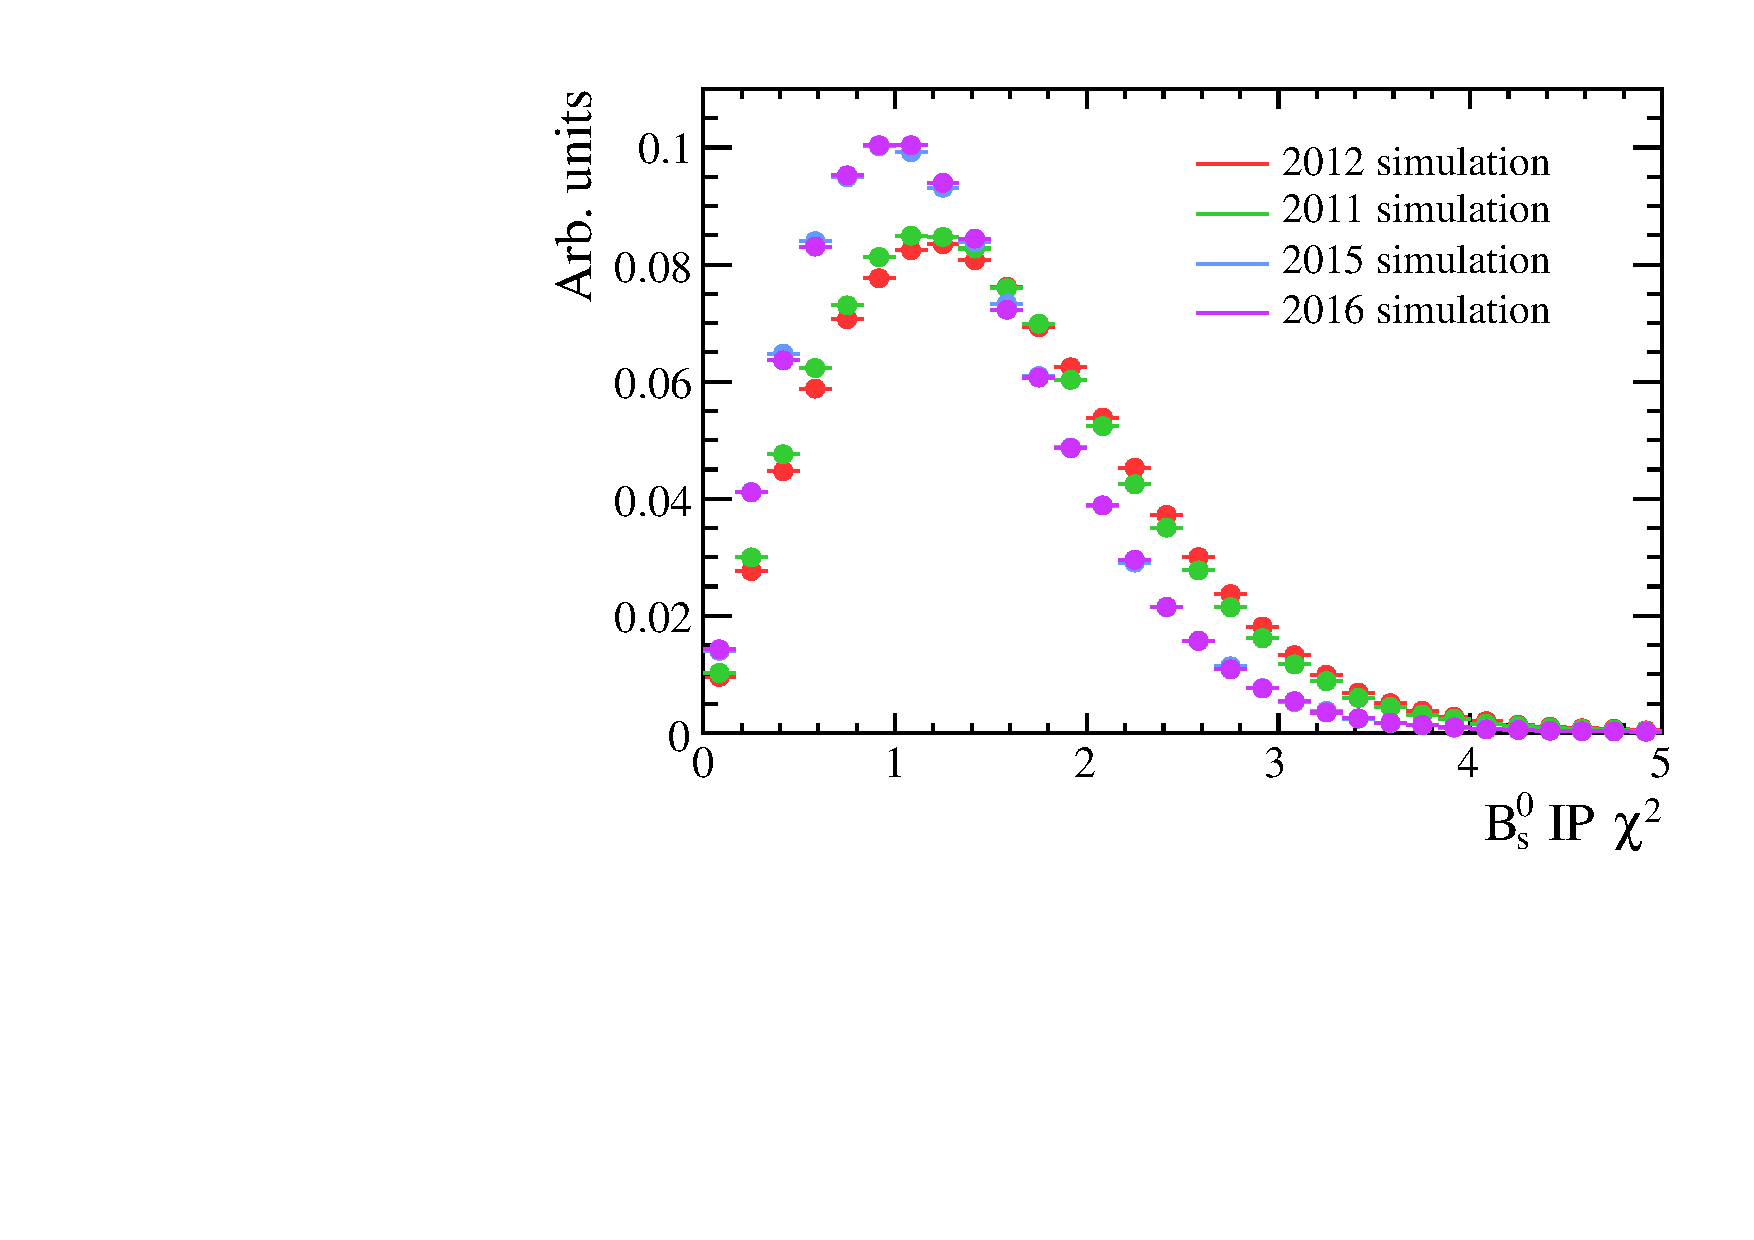
\includegraphics[width=\textwidth]{./Figs/Selection/signal_IPS.pdf}
        \caption{ }
        \label{fig:BDTbkg}
    \end{subfigure}





 \begin{subfigure}[b]{0.48\textwidth}
        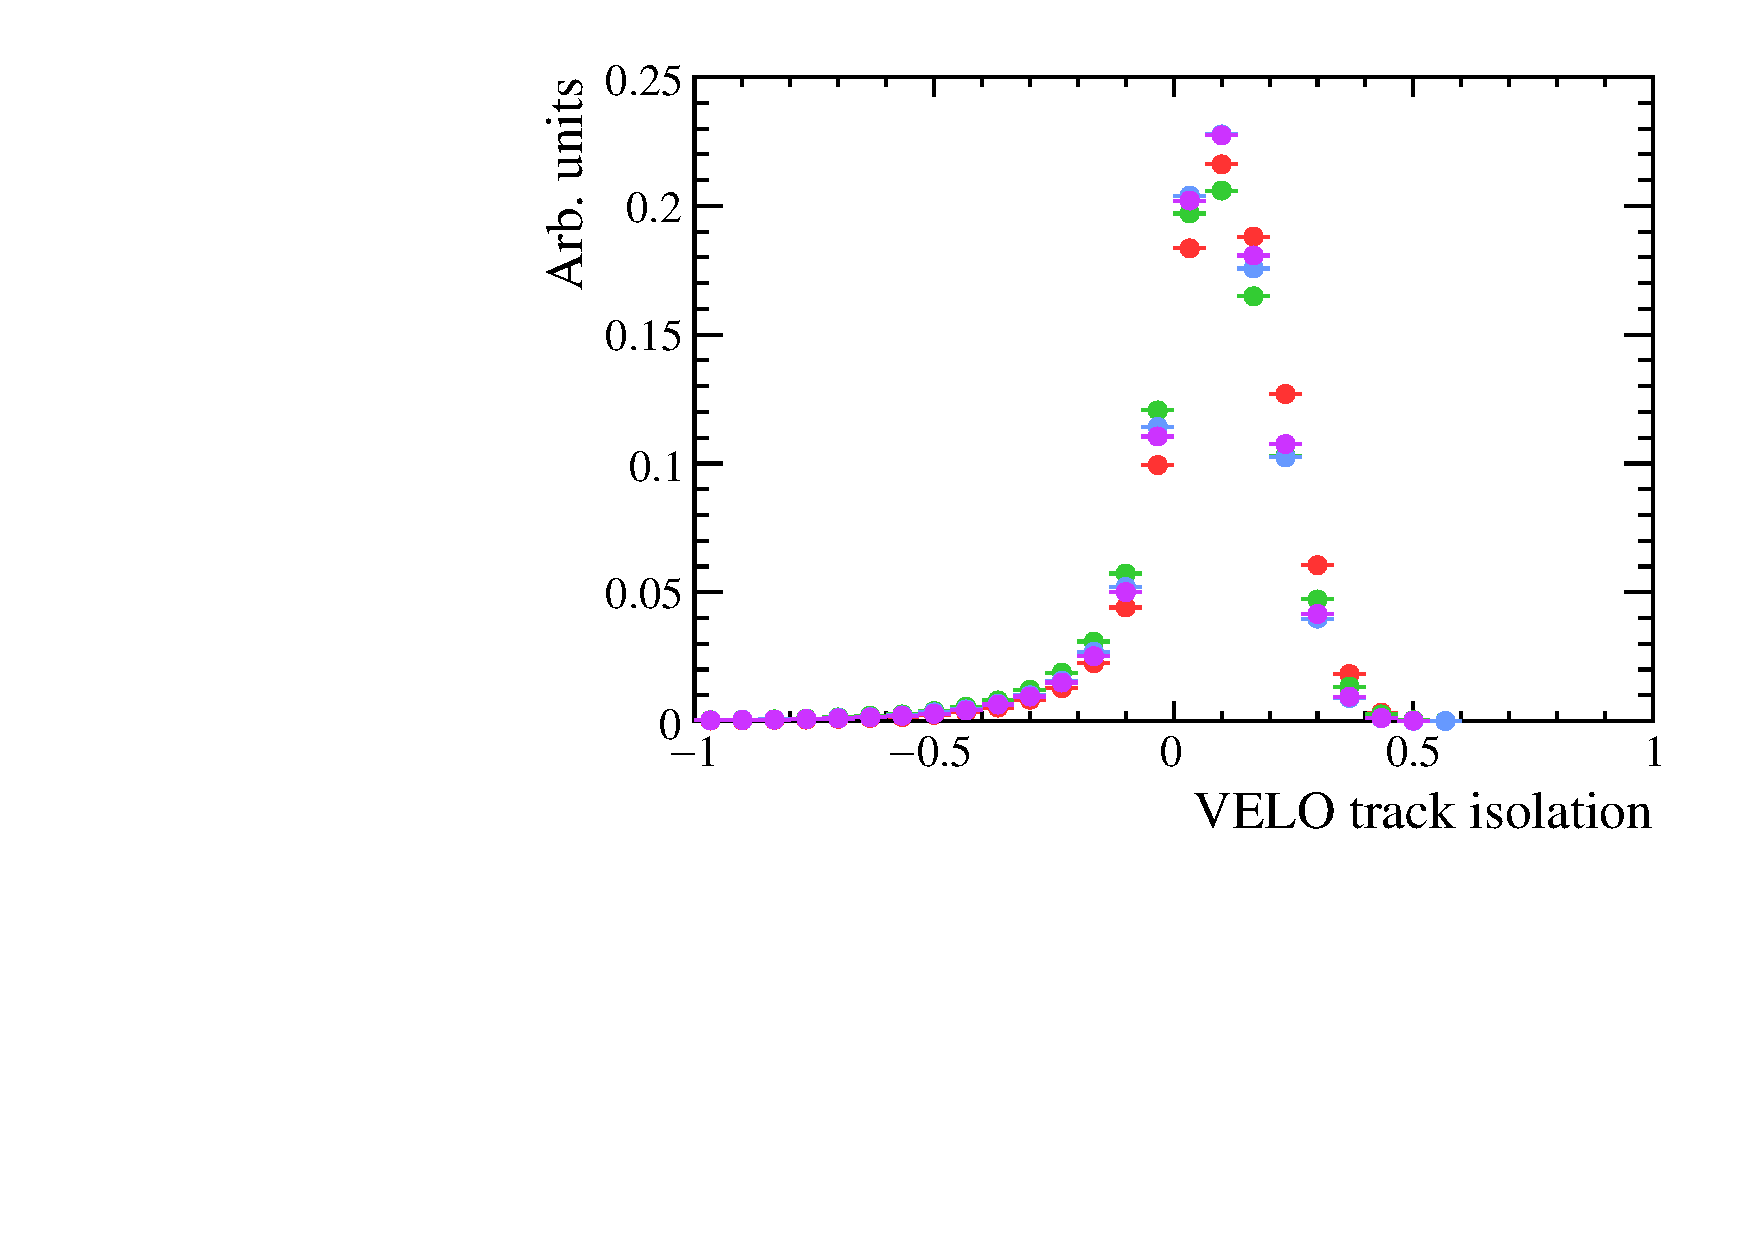
\includegraphics[width=\textwidth]{./Figs/Selection/signal_iso_velo.pdf}
        \caption{ }
        \label{fig:BDTsig}
    \end{subfigure}
    ~ %add desired spacing between images, e. g. ~, \quad, \qquad, \hfill etc. 
      %(or a blank line to force the subfigure onto a new line)
    \begin{subfigure}[b]{0.48\textwidth}
       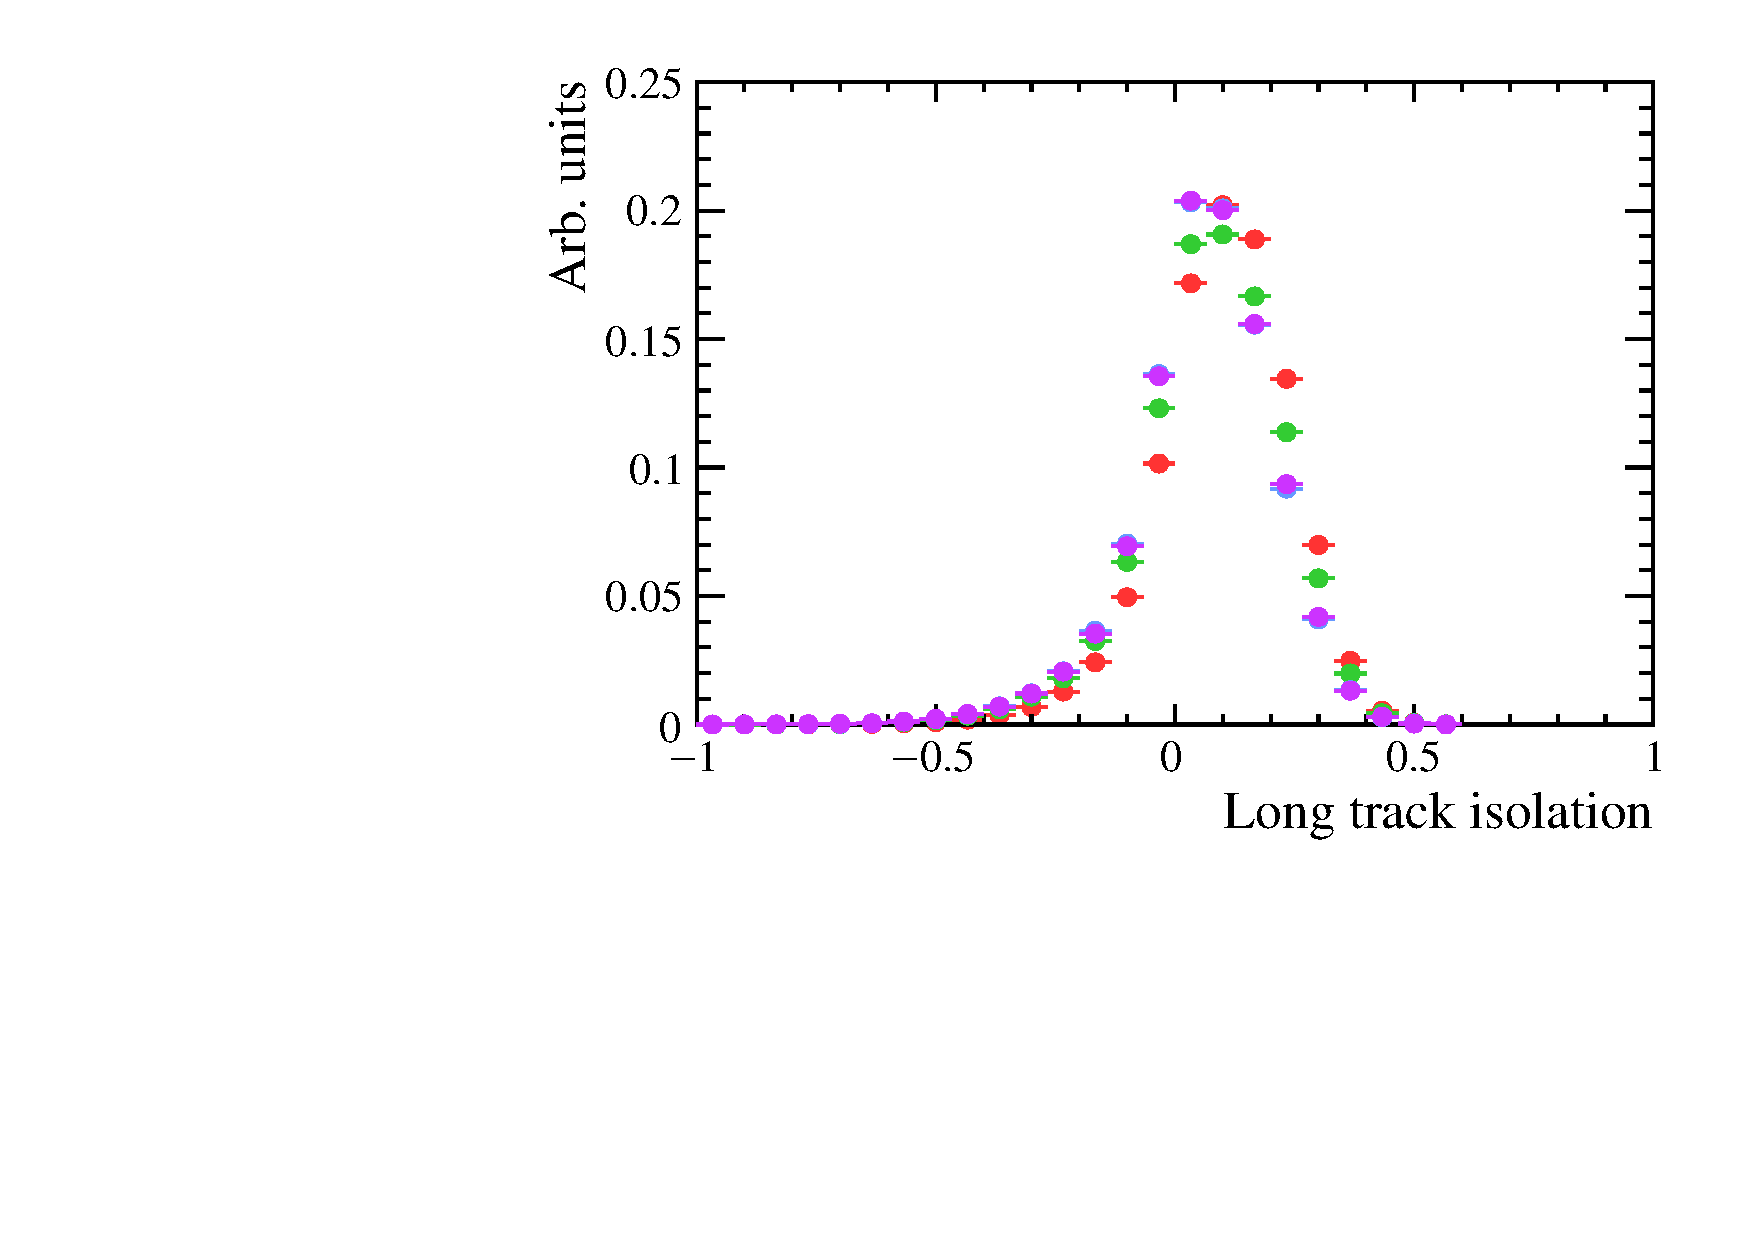
\includegraphics[width=\textwidth]{./Figs/Selection/signal_long_iso.pdf}
        \caption{ }
        \label{fig:BDTbkg}
    \end{subfigure}




 \begin{subfigure}[b]{0.48\textwidth}
        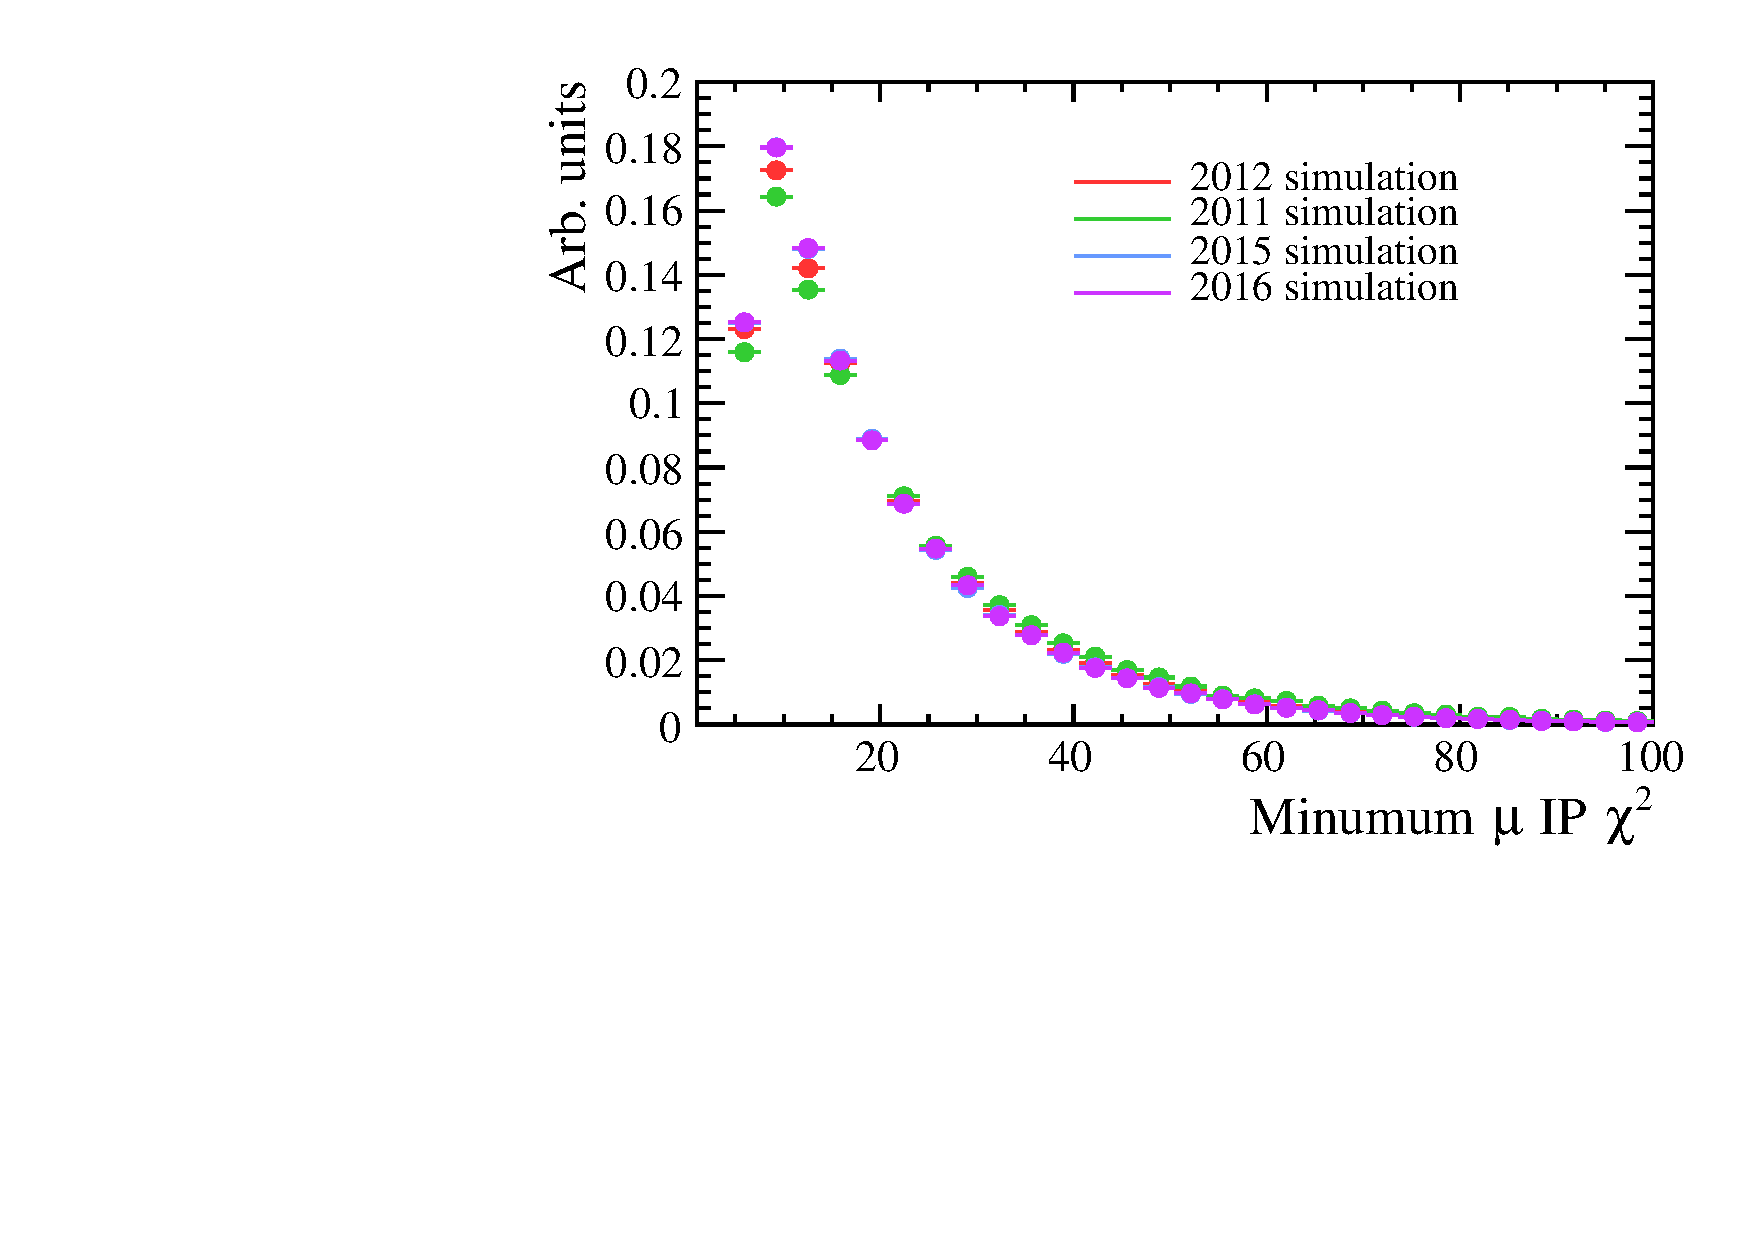
\includegraphics[width=\textwidth]{./Figs/Selection/signal_muIPS.pdf}
        \caption{ }
        \label{fig:BDTsig}
    \end{subfigure}
    ~ %add desired spacing between images, e. g. ~, \quad, \qquad, \hfill etc. 
      %(or a blank line to force the subfigure onto a new line)
 



    \caption{Signal distribution for input variables for the global BDT for \bsmumu simulated decays in 2011, 2012, 2015 and 2016.}
    \label{fig:signalvars}
\end{figure}



\begin{figure}
    \centering
    \begin{subfigure}[b]{0.48\textwidth}
        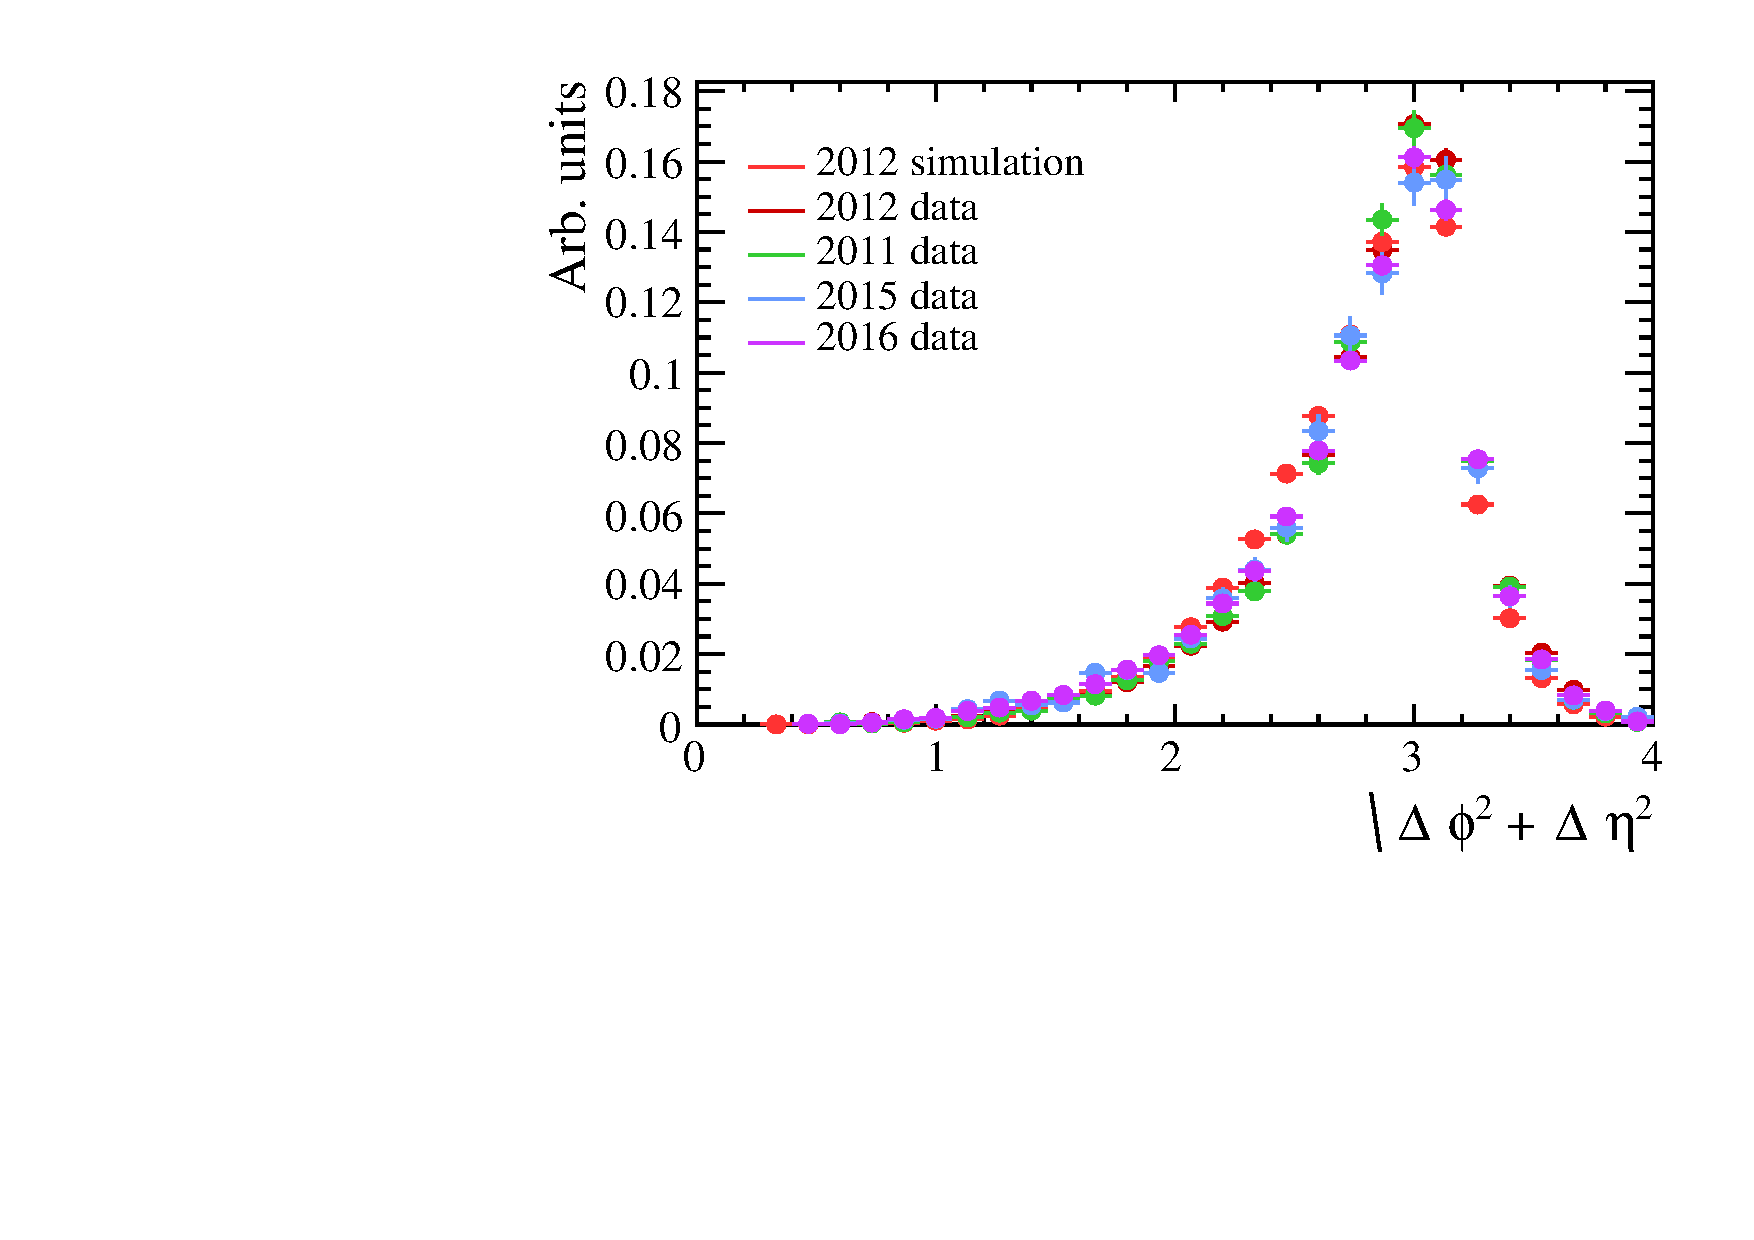
\includegraphics[width=\textwidth]{./Figs/Selection/bkgnf_DeltaR.pdf}
        \caption{ }
        \label{fig:BDTsig}
    \end{subfigure}
    ~ %add desired spacing between images, e. g. ~, \quad, \qquad, \hfill etc. 
      %(or a blank line to force the subfigure onto a new line)
    \begin{subfigure}[b]{0.48\textwidth}
       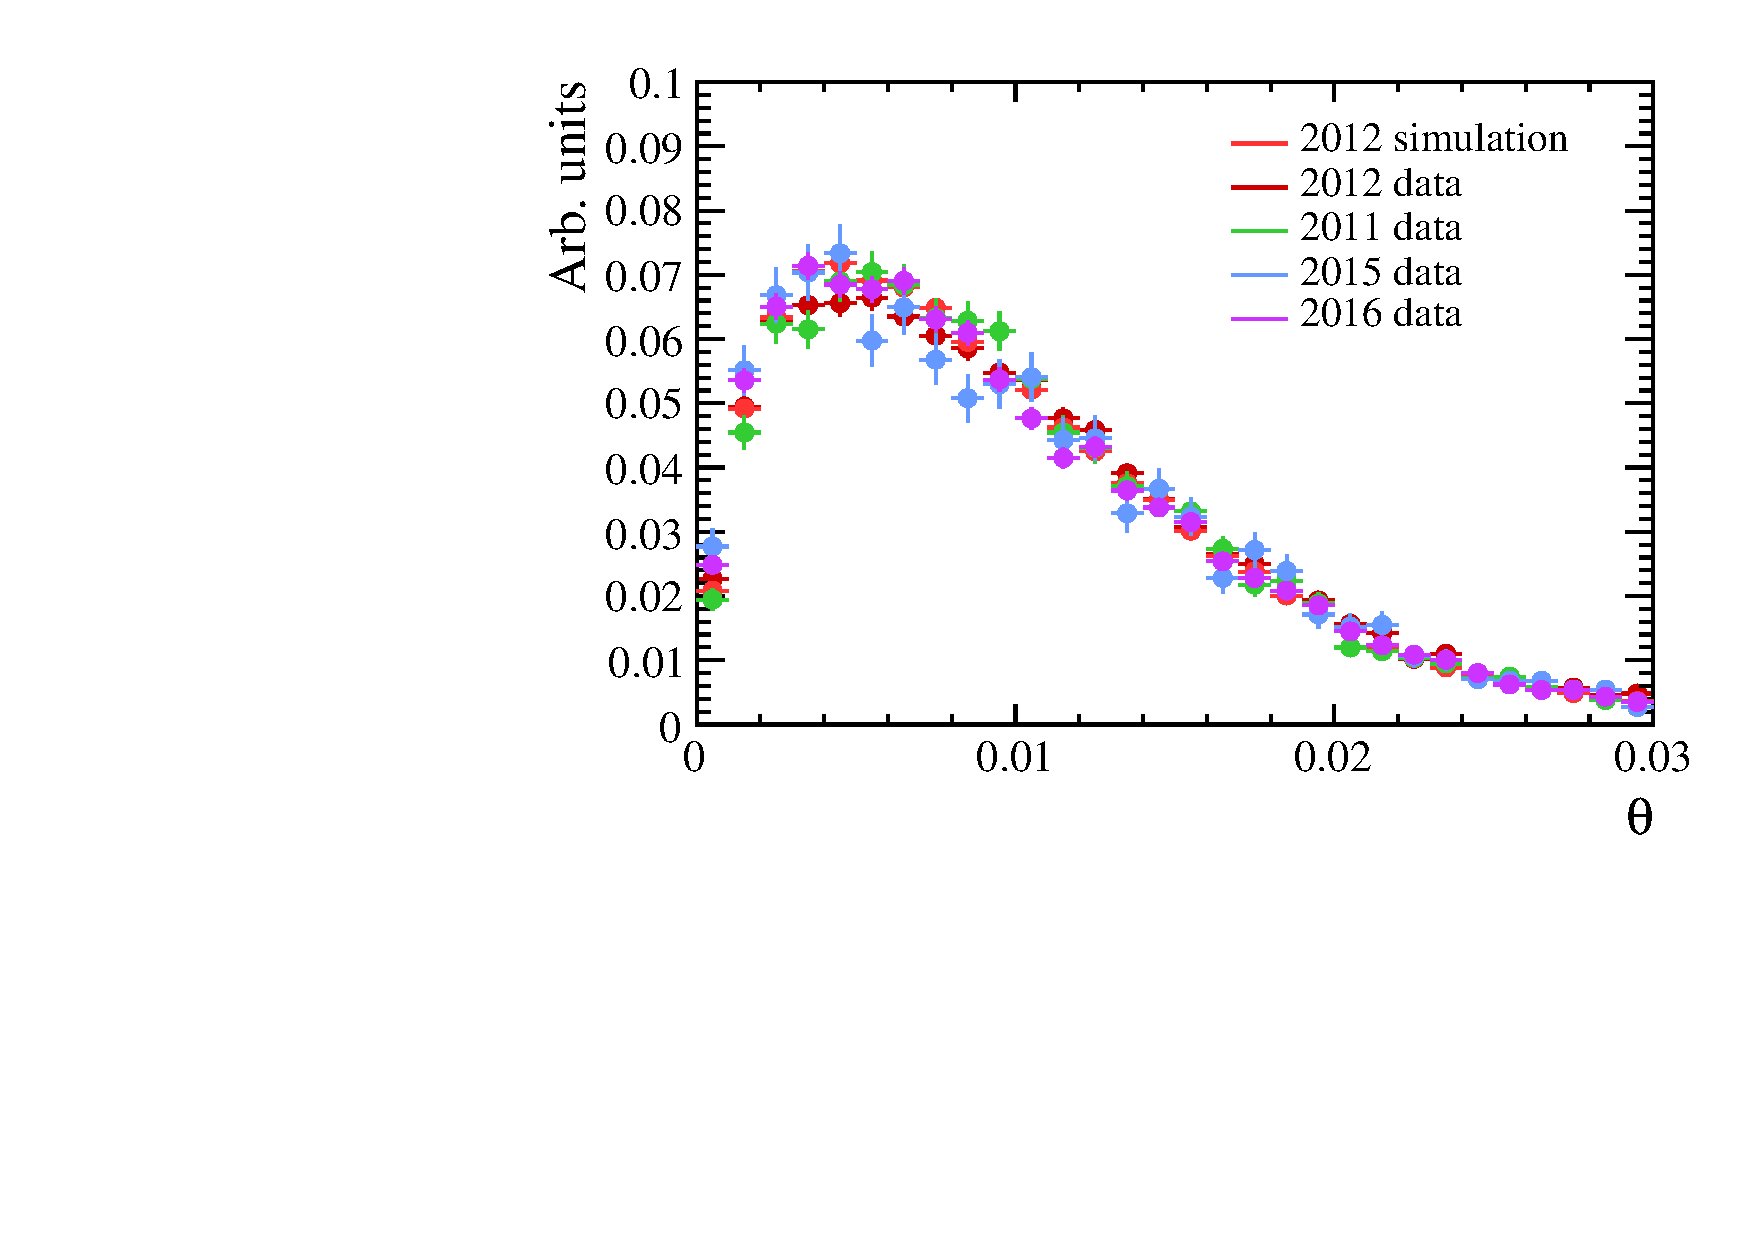
\includegraphics[width=\textwidth]{./Figs/Selection/bkgnd_DIRA.pdf}
        \caption{ }
        \label{fig:BDTbkg}
    \end{subfigure}



 \begin{subfigure}[b]{0.48\textwidth}
        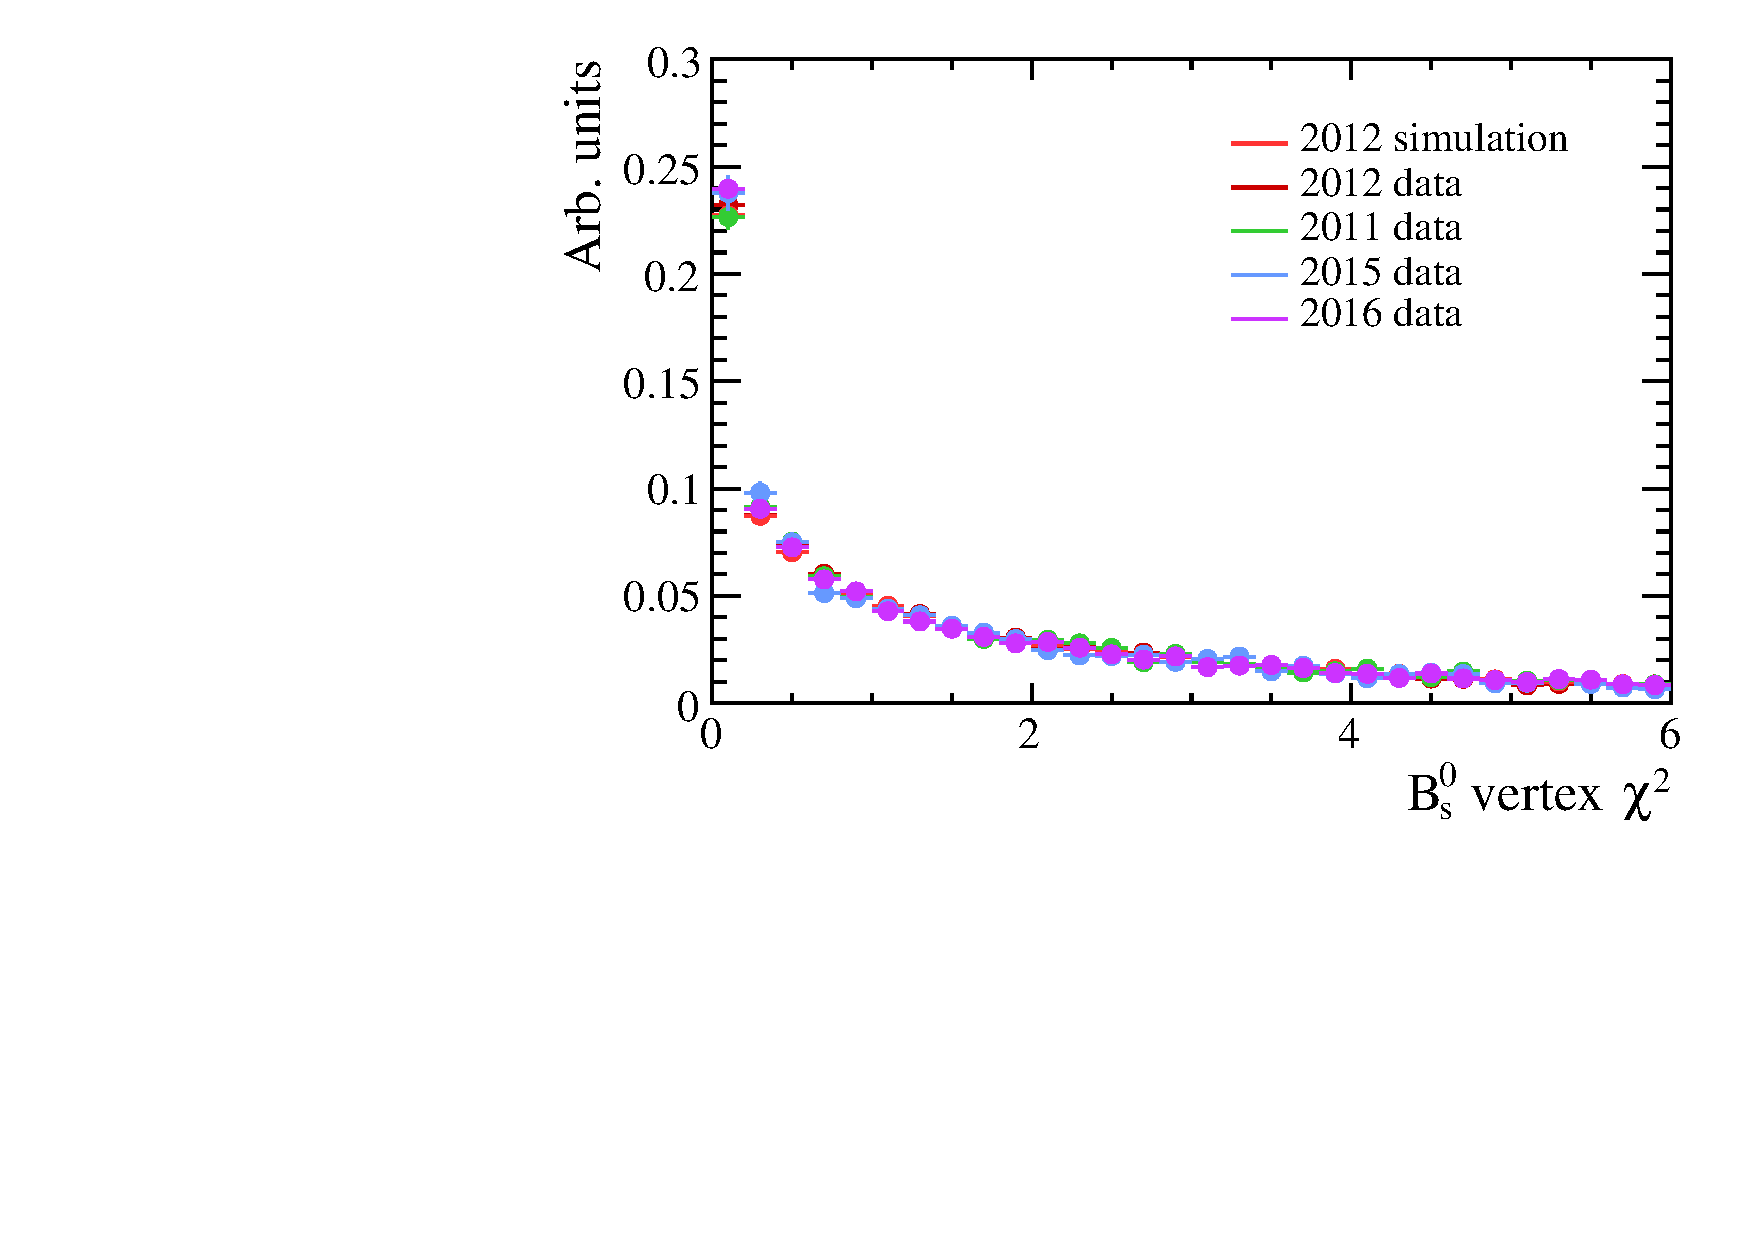
\includegraphics[width=\textwidth]{./Figs/Selection/bkgnd_vertex.pdf}
        \caption{ }
        \label{fig:BDTsig}
    \end{subfigure}
    ~ %add desired spacing between images, e. g. ~, \quad, \qquad, \hfill etc. 
      %(or a blank line to force the subfigure onto a new line)
    \begin{subfigure}[b]{0.48\textwidth}
       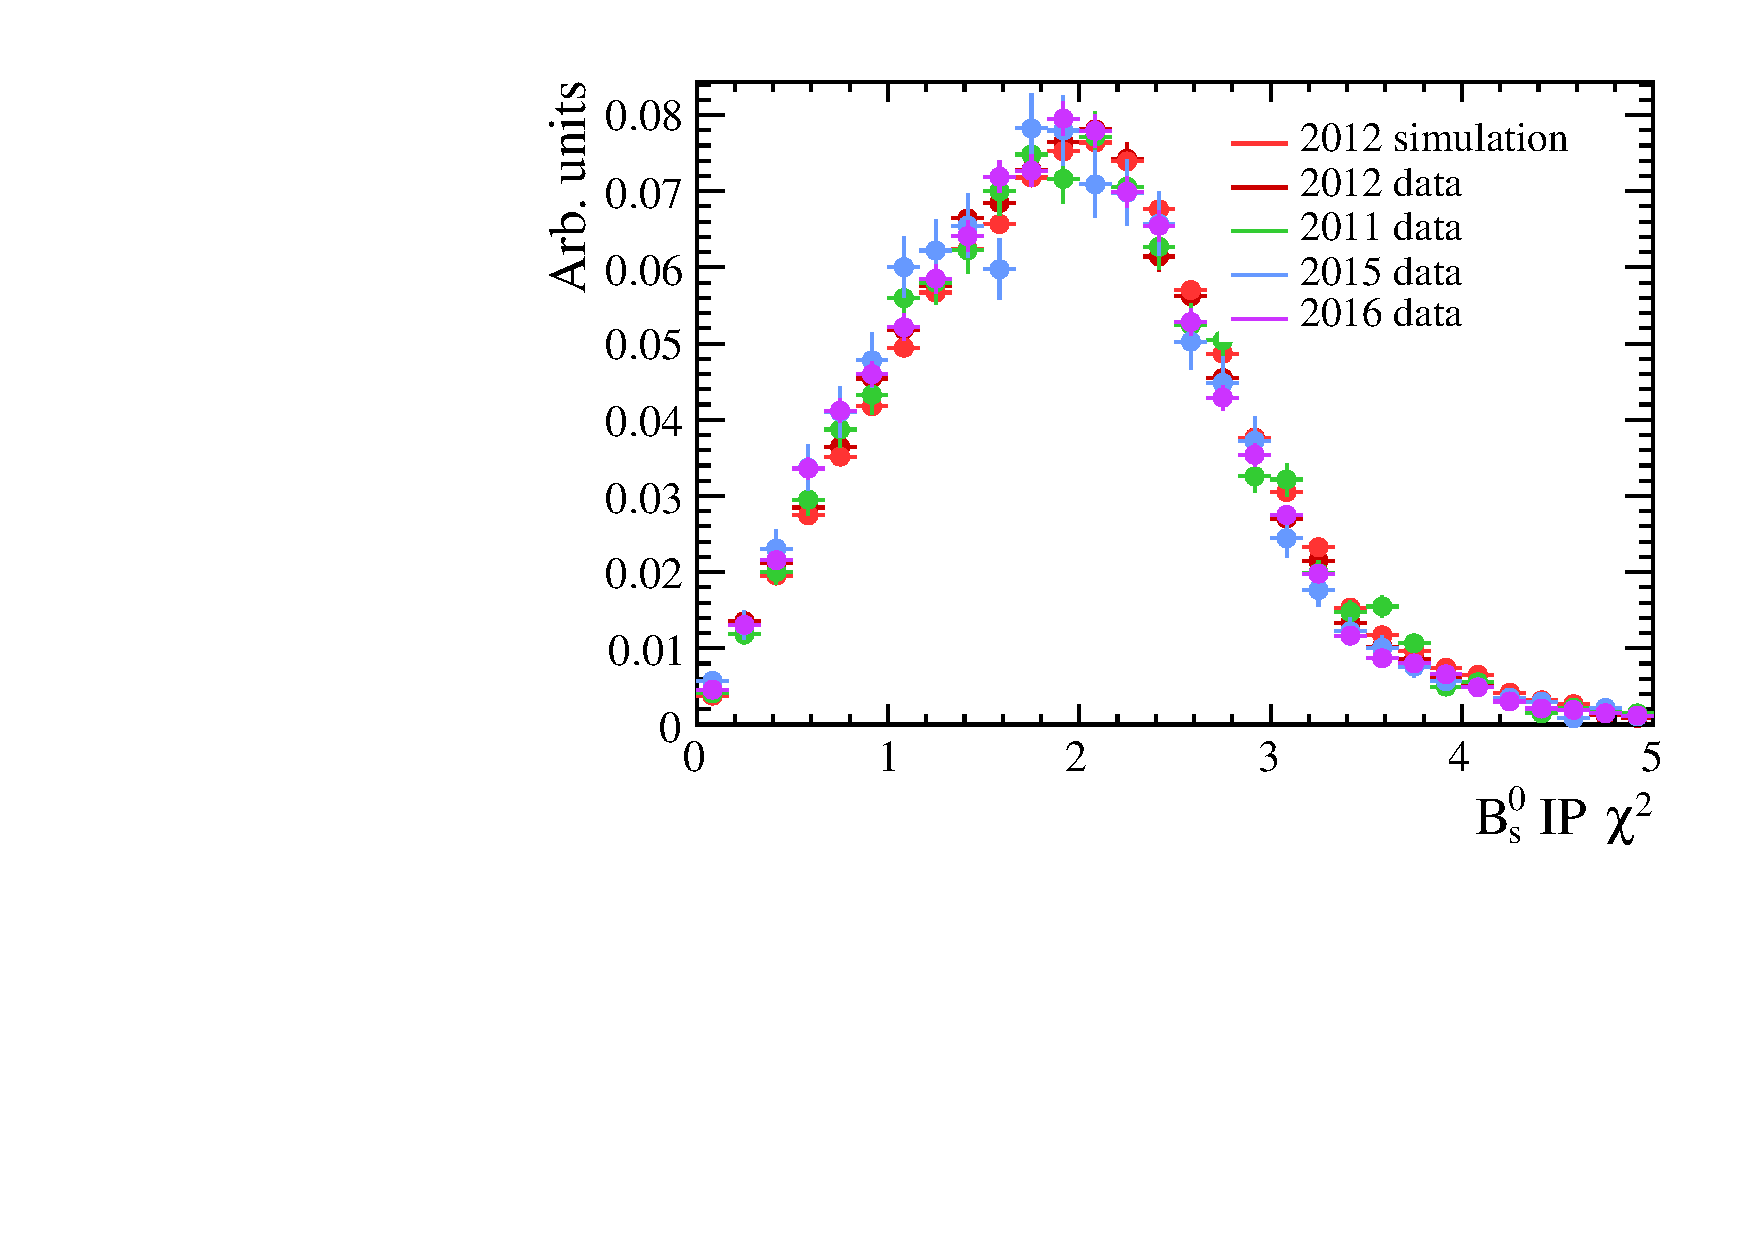
\includegraphics[width=\textwidth]{./Figs/Selection/bkgnd_IPS.pdf}
        \caption{ }
        \label{fig:BDTbkg}
    \end{subfigure}





 \begin{subfigure}[b]{0.48\textwidth}
        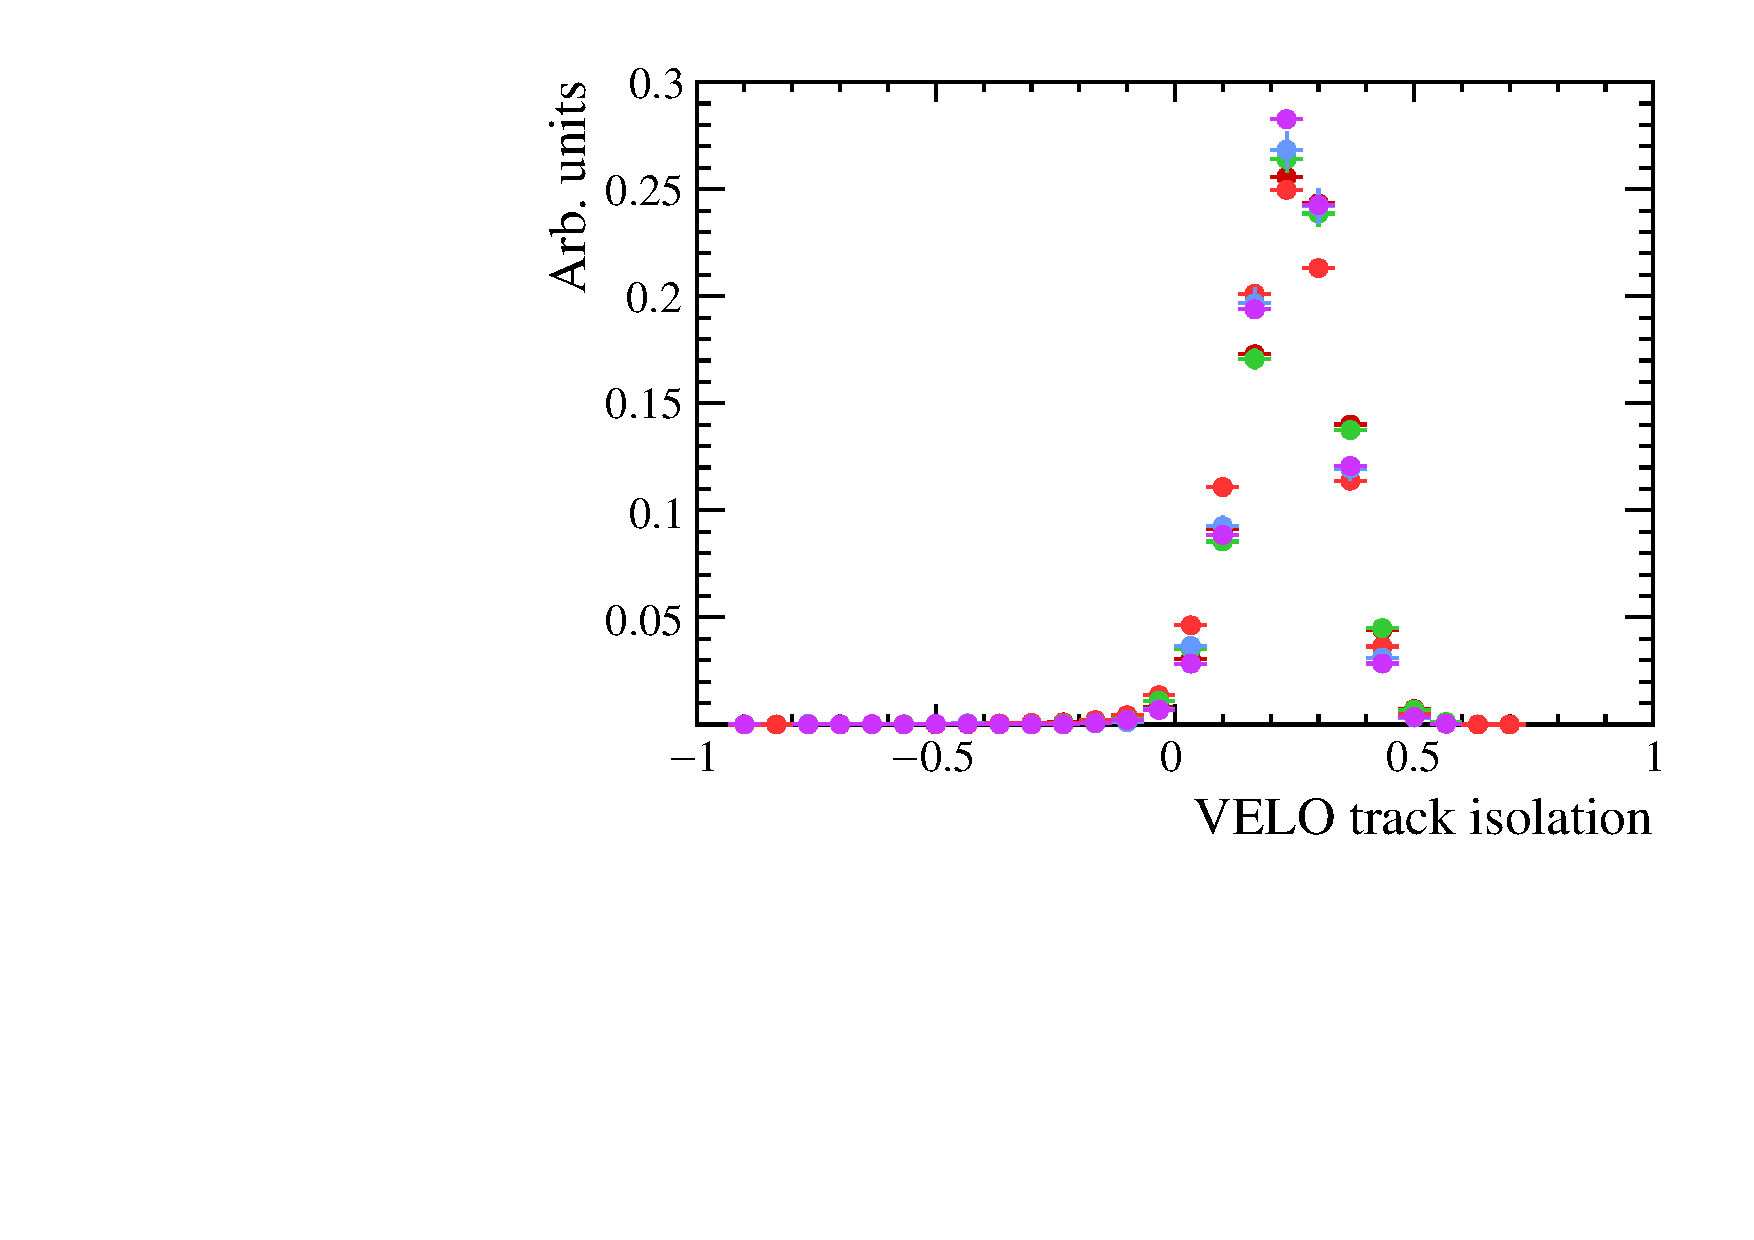
\includegraphics[width=\textwidth]{./Figs/Selection/bkgnd_iso_velo.pdf}
        \caption{ }
        \label{fig:BDTsig}
    \end{subfigure}
    ~ %add desired spacing between images, e. g. ~, \quad, \qquad, \hfill etc. 
      %(or a blank line to force the subfigure onto a new line)
    \begin{subfigure}[b]{0.48\textwidth}
       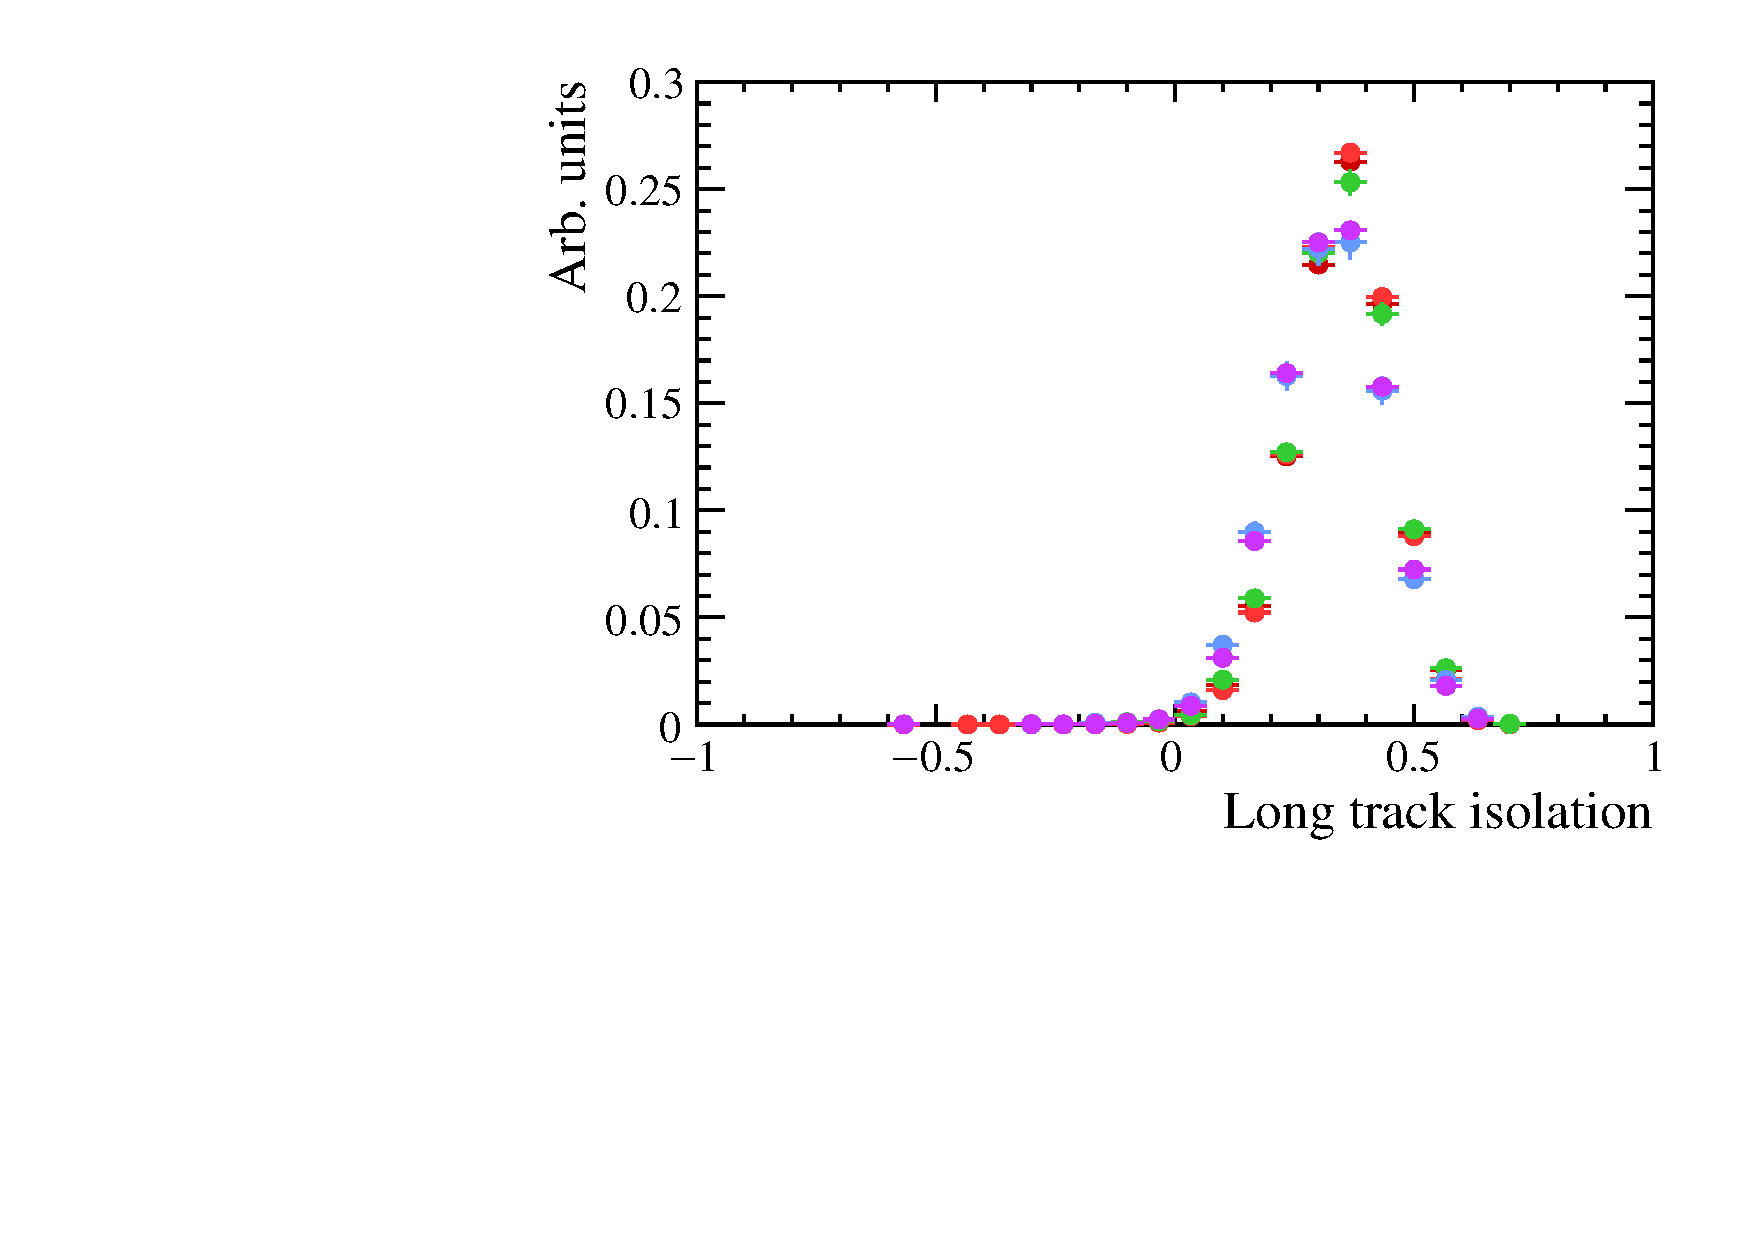
\includegraphics[width=\textwidth]{./Figs/Selection/bkgnd_long_iso.pdf}
        \caption{ }
        \label{fig:BDTbkg}
    \end{subfigure}




 \begin{subfigure}[b]{0.48\textwidth}
        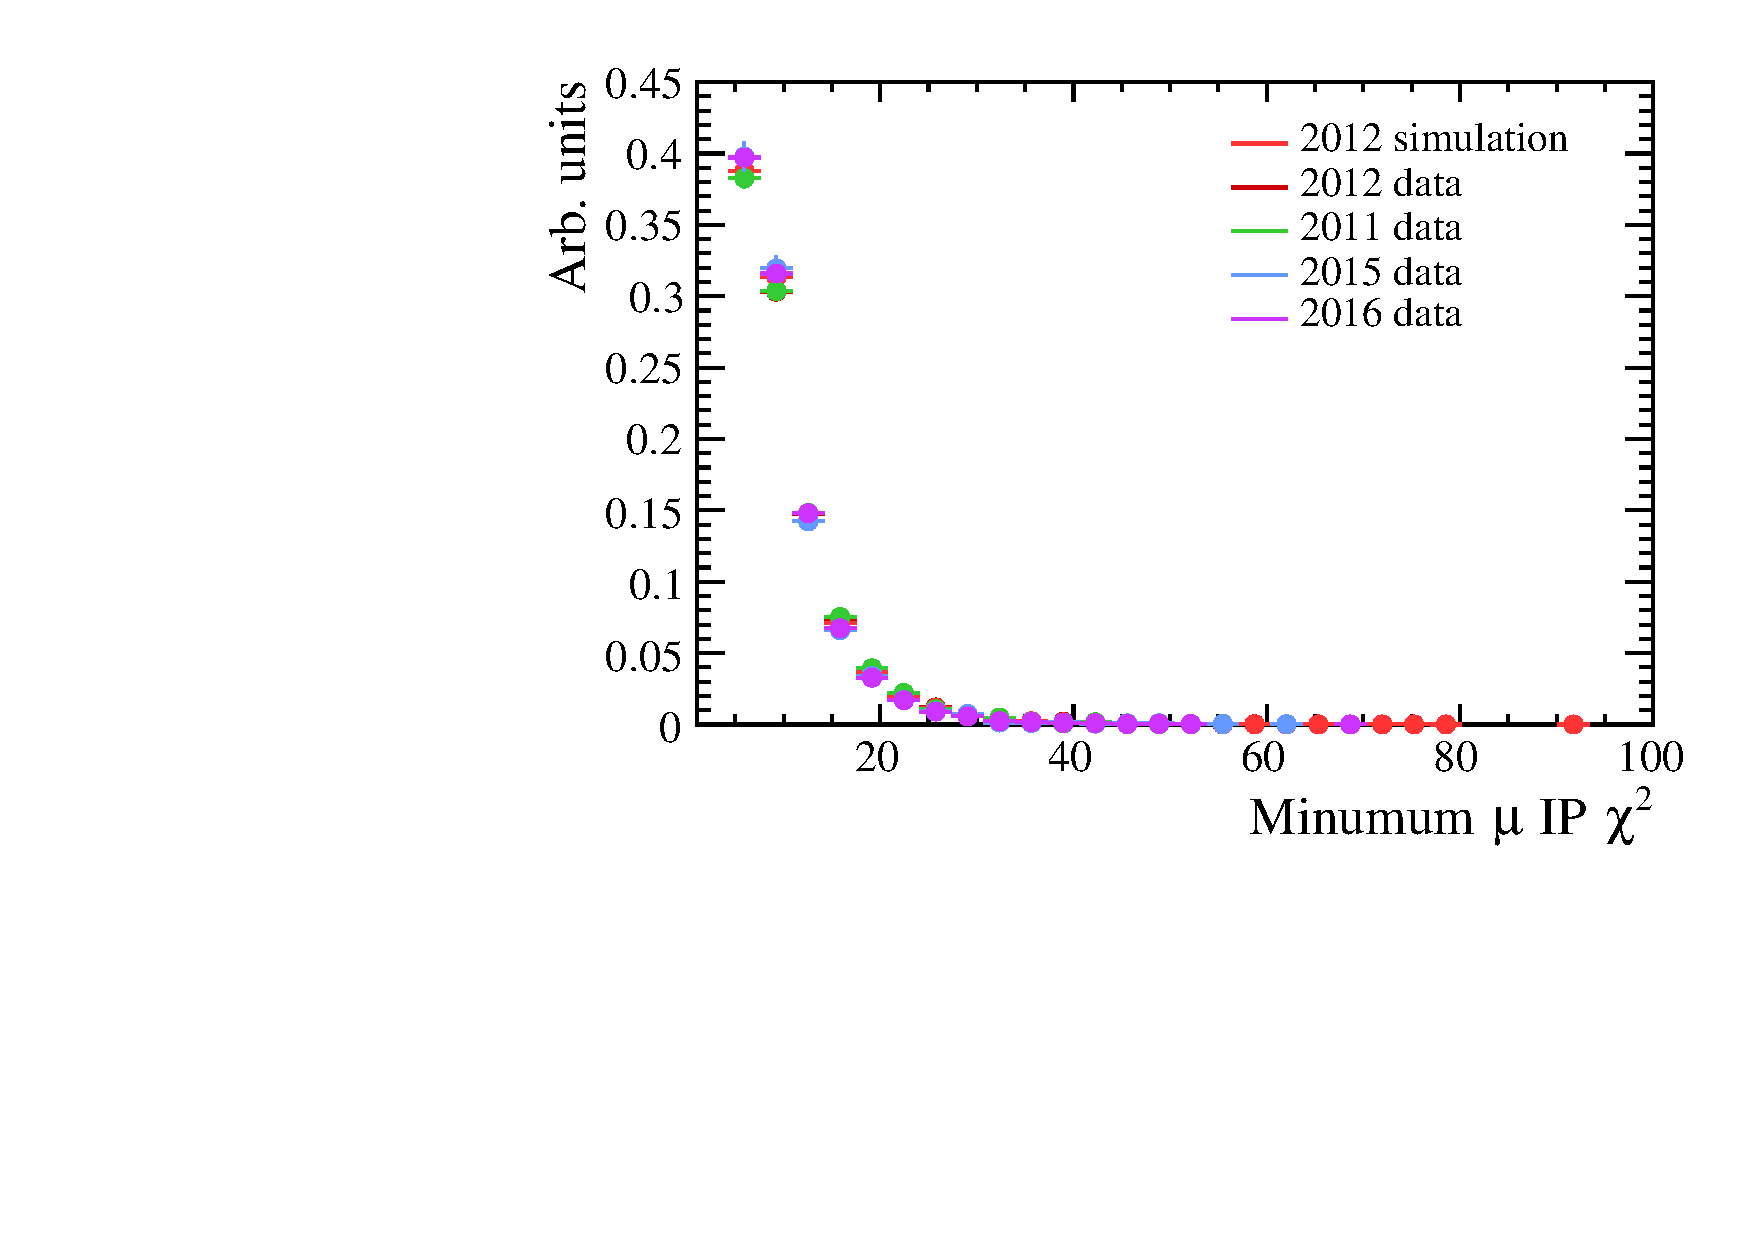
\includegraphics[width=\textwidth]{./Figs/Selection/bkgnd_muIPS.pdf}
        \caption{ }
        \label{fig:BDTsig}
    \end{subfigure}
    ~ %add desired spacing between images, e. g. ~, \quad, \qquad, \hfill etc. 
      %(or a blank line to force the subfigure onto a new line)
 



    \caption{Background distribution for input variables from \bbbbarmumux decays in 2011, 2012, 2015 and 2016 data with $m_{\mu \mu} > 5447$ \mevcc and 2012 simulated \bbbbarmumux decays.}
    \label{fig:signalvars}
\end{figure}
